%%%%%%%%%%%%%%%%%%%%%%%%%%%%%%%%%%%%%%%%%%%%%%%%%%%%%%%%%%%%%%%%%%%
%                                                                 %                    
%                 Packages / Grundeinstellungen                   %
%                                                                 %
%%%%%%%%%%%%%%%%%%%%%%%%%%%%%%%%%%%%%%%%%%%%%%%%%%%%%%%%%%%%%%%%%%%
\DocumentMetadata{
    pdfversion=2.0,
    pdfstandard=A-4,
}

\documentclass[paper=a1,parskip=half,fontsize=24]{scrartcl}

\usepackage[ngerman]{babel}
\usepackage{lmodern}
\usepackage{fontspec}
\usepackage{calc}
\usepackage{microtype}
\usepackage{tcolorbox}
\usepackage{blindtext}
\usepackage{float}
\usepackage{subcaption}

% Keine floats in andere Sections
\usepackage[section]{placeins}

% Eurozeichen einbinden
\usepackage[right]{eurosym}

% Floatende Bilder ermöglichen
\usepackage{floatflt}

% Bricht lange URLs "schön" um
\usepackage[hyphens,obeyspaces,spaces]{url}

% Mathematische Symbole importieren
\usepackage{amssymb}

% Zitierung nach APA
%\usepackage[
%backend=biber,
%style=apa,
%autocite=inline,
%]{biblatex}
%\addbibresource{bibtex/poster.bib}

% Zitierung nach IEEE
\usepackage[
backend=biber,
style=ieee,
autocite=inline,
]{biblatex}
\addbibresource{bibtex/poster.bib}

\setcounter{biburllcpenalty}{7000}
\setcounter{biburlucpenalty}{8000}

% Paket für Zeilenabstand
\usepackage{setspace}

% Für Bildbezeichner
\usepackage{capt-of}

% Für Stichwortverzeichnis
\usepackage{makeidx}

% Erzeugt Inhaltsverzeichnis mit Querverweisen zu den Abschnitten (PDF Version)
\usepackage[bookmarksnumbered,hyperfootnotes=false,hypertexnames=false]{hyperref}
\hypersetup{
  colorlinks=true,
  linkcolor=black,
  filecolor=blue,
  citecolor = black,      
  urlcolor=blue,
  }

%mehrspaltig
\usepackage{multicol} 
\columnsep=70pt 
\columnseprule=3pt 

%grafiken einbinden
\usepackage{graphicx}

% Booktabs Tabellen
\usepackage{tabularray}
\UseTblrLibrary{booktabs}
\DefTblrTemplate{contfoot-text}{normal}{Fortsetzung auf nächster Seite}
\SetTblrTemplate{contfoot-text}{normal}
\DefTblrTemplate{conthead-text}{normal}{}
\SetTblrTemplate{conthead-text}{normal}

% Paket für Textfarben
\usepackage{xcolor} 
\definecolor{LightGray}{gray}{0.9}
\usepackage[pagecolor=white]{pagecolor}
\usepackage{listings}
 \usepackage{fontspec}

 \lstset{
 basicstyle=\treefont\footnotesize,
   columns=fixed,
   keepspaces=true,
   breaklines=false,
   extendedchars=true,
    aboveskip=0pt,
  belowskip=0pt
   }

 \newfontfamily\treefont{DejaVu Sans Mono}
% Für schönere Listings
\usepackage[newfloat,]{minted}
\setminted{
  frame=lines,
  framesep=2mm,
  baselinestretch=1.2,
  bgcolor=LightGray,
  fontsize=\footnotesize,
  linenos,
  breaklines=true,
  breakanywhere=true,
  autogobble,
  tabsize=2
}
\setmintedinline{}
\usepackage{caption}
% Keine Floats bei Listings
\newenvironment{code}[2]
  {
  \providecommand{\captiontitle}{#1}
  \providecommand{\labeltitle}{#2}
  \vspace*{0.3cm}
  }
  {
  %\vspace*{-2.0cm}
  \captionbelowof{listing}{\captiontitle}
  \label{\labeltitle}
  \vspace*{0.35cm}
  }
\SetupFloatingEnvironment{listing}{}

%seitengeometrie
\usepackage{geometry}
\geometry{margin=3cm,top=3cm}

%Definition Schrift- und Farbeinstellungen 
\setmainfont{TeX Gyre Termes}
\setsansfont{TeX Gyre Adventor}
\usepackage{preamble}


%Siehe hierzu preamble.sty
\colorlet{basecolor}{violet}
\colorlet{akzentcolor}{mint}

%Siehe hierzu preamble.sty
\renewcommand{\theauthor}{Team-h: Joliesse Ludivine Magne Tuekam, Danielle Grace Matcheu Youmssi, Joyce Markline Sambou Leundja, Joslyno Azemgning}
\renewcommand{\thetitle}{Bibliothekanwendung-Damas}
\renewcommand{\thesubtitle}{Entwicklung einer Webanwendung}

%Höhe des HS Logos 4cm für zweizeiligen Titel, 2.5cm für einzeiligen Titel
\newcommand{\myspace}{4cm}

\hypersetup{pdfinfo={
  Title={\thetitle},
  Author={\theauthor}
}}

% Darf erst hier eingebunden werden! 
\usepackage{csquotes}

%Textfarbe
\color{black}

%%%%%%%%%%%%%%%%%%%%%%%%%%%%%%%%%%%%%%%%%%%%%%%%%%%%%%%%%%%%%%%%%%%
%                                                                 %                    
%                     Beginn des Inhalts                          %
%                                                                 %
%%%%%%%%%%%%%%%%%%%%%%%%%%%%%%%%%%%%%%%%%%%%%%%%%%%%%%%%%%%%%%%%%%%

%%%%%%%%%%%%%%%%%%%%%%%%%%%%%%%%%%%%%%%%%%%%%%%%%%%%%%%%%%%%%%%%%%%
%  Special Characters:                                            %
%                                                                 %
%             \& \% \$ \# \_ \{ \}                                %
%             \textasciitilde (~)                                 %
%             \textasciicircum (^)                                %     
%             \textbackslash (\)                                  %                    
%      \glqq Text\grqq{} für Anführungszeichen                    %
%%%%%%%%%%%%%%%%%%%%%%%%%%%%%%%%%%%%%%%%%%%%%%%%%%%%%%%%%%%%%%%%%%%


\begin{document}
  %Printed Überschriften
  \thetitlearea
  %Mehrspaltig
  \begin{multicols*}{3}
  
    % Input Inhalt
    \section{Einleitung und Beschreibung des Projekts}

\subsection{Einleitung}

In „Software Engineering II“ haben wir auf den bisher erlernten Grundlagen aufgebaut und unser Verständnis für zentrale Aspekte der Softwareentwicklung vertieft – von der Entwicklungsumgebung über Nebenläufigkeit und Datenbankanbindung bis hin zur systematischen Problemfindung. Ein besonderer Fokus lag auf der Vertiefung objektorientierter Konzepte: Durch die intensive Arbeit mit dem Jakarta-Servlet-API, Vererbung und Design Patterns haben wir gelernt, wiederverwendbaren und gut strukturierten Code zu schreiben, der uns zugleich hilft, Probleme systematisch zu analysieren und im Team zu lösen.

Im Folgenden präsentieren wir die Ergebnisse der Semesteraufgabe: eine Bibliotheksanwendung, die es Mitarbeitern ermöglicht, sich anzumelden und zwischen den Anwendungsfällen Ausleihe und Rückgabe zu wählen. Über die geforderten Kernfunktionen hinaus haben wir eine eigenständige Registrierung für Mitglieder ergänzt, die eng mit dem bestehenden Login-System verzahnt ist, sodass neu registrierte Mitglieder unmittelbar im System anmelden und ihre Ausleihen einsehen können.

\subsection{Beschreibung des Projekts}

Den Kern der Anwendung bilden die beiden geforderten Anwendungsfälle Ausleihe und Rückgabe. Mitarbeiter geben dabei zunächst den Ausweiscode eines Mitglieds ein, gefolgt von einer beliebigen Anzahl an Buchexemplar-Codes, die per Tastatur eingegeben werden, um einen Barcode-Scanner zu simulieren. Erst nach ausdrücklicher Bestätigung der vollständigen Erfassung wird die Ausleihe beziehungsweise Rückgabe tatsächlich in der Datenbank festgehalten. Bestätigungsdokumente werden dabei nicht unmittelbar geschrieben, sondern als eigenständiges Objekt gekapselt und in eine Redis-Warteschlange eingereiht; ein separater, nebenläufig laufender Prozess entnimmt diese Aufträge und schreibt die entsprechenden Quittungen als Textdateien.

Über die Kernfunktionen hinaus haben wir die Anwendung um mehrere Module erweitert, die reale Bibliotheksprozesse abbilden: Bei der Inventur erfassen Mitarbeiter Buchexemplare je Standort, wobei das System automatisch über- sowie unterzählige Bestände ermittelt; ein Mitglieder-Dashboard zeigt die eigene Ausleih-Historie, während ein administrativer Bereich Bestand und Anschaffungen verwaltet. Zur Sicherung der Codequalität haben wir zudem einen Git-Hook eingerichtet, der falsch formatierten Java-Code bereits vor dem Push zurückweist, und den vollständigen Ablauf von Anmeldung über eine Aktion bis zur Abmeldung als Grundlage für einen nebenläufigen Lasttest genutzt, dessen Ergebnisse wir visualisiert und ausgewertet haben.
Für die Entwicklung der Benutzeroberfläche wurden HTML, CSS und JavaScript verwendet \autocite{w3school}.
 \autocite{JavaDoc}.

    \section{Anforderungsanalyse}

\subsection{Stakeholder}
Im Rahmen der Bibliotheksanwendung lassen sich folgende Stakeholder identifizieren:
\\\textbf{Mitglieder} -- Nutzer der Bibliothek, die Bücher ausleihen, zurückgeben und ihren Kontostatus einsehen möchten.
\\\textbf{Mitarbeiterinnen und Mitarbeiter} -- Bibliothekspersonal, das Ausleihen und Rückgaben durchführt, Mitglieder verwaltet und bei Bedarf sperren oder freigeben kann.
\\\textbf{Administratorinnen und Administratoren} -- Mitarbeitende mit erweiterten Rechten, die Statistiken einsehen, Bücher verwalten und Auswertungen durchführen können.

\subsection{Personas}
\begin{figure}[H]
\vspace{-10pt}
  \centering
   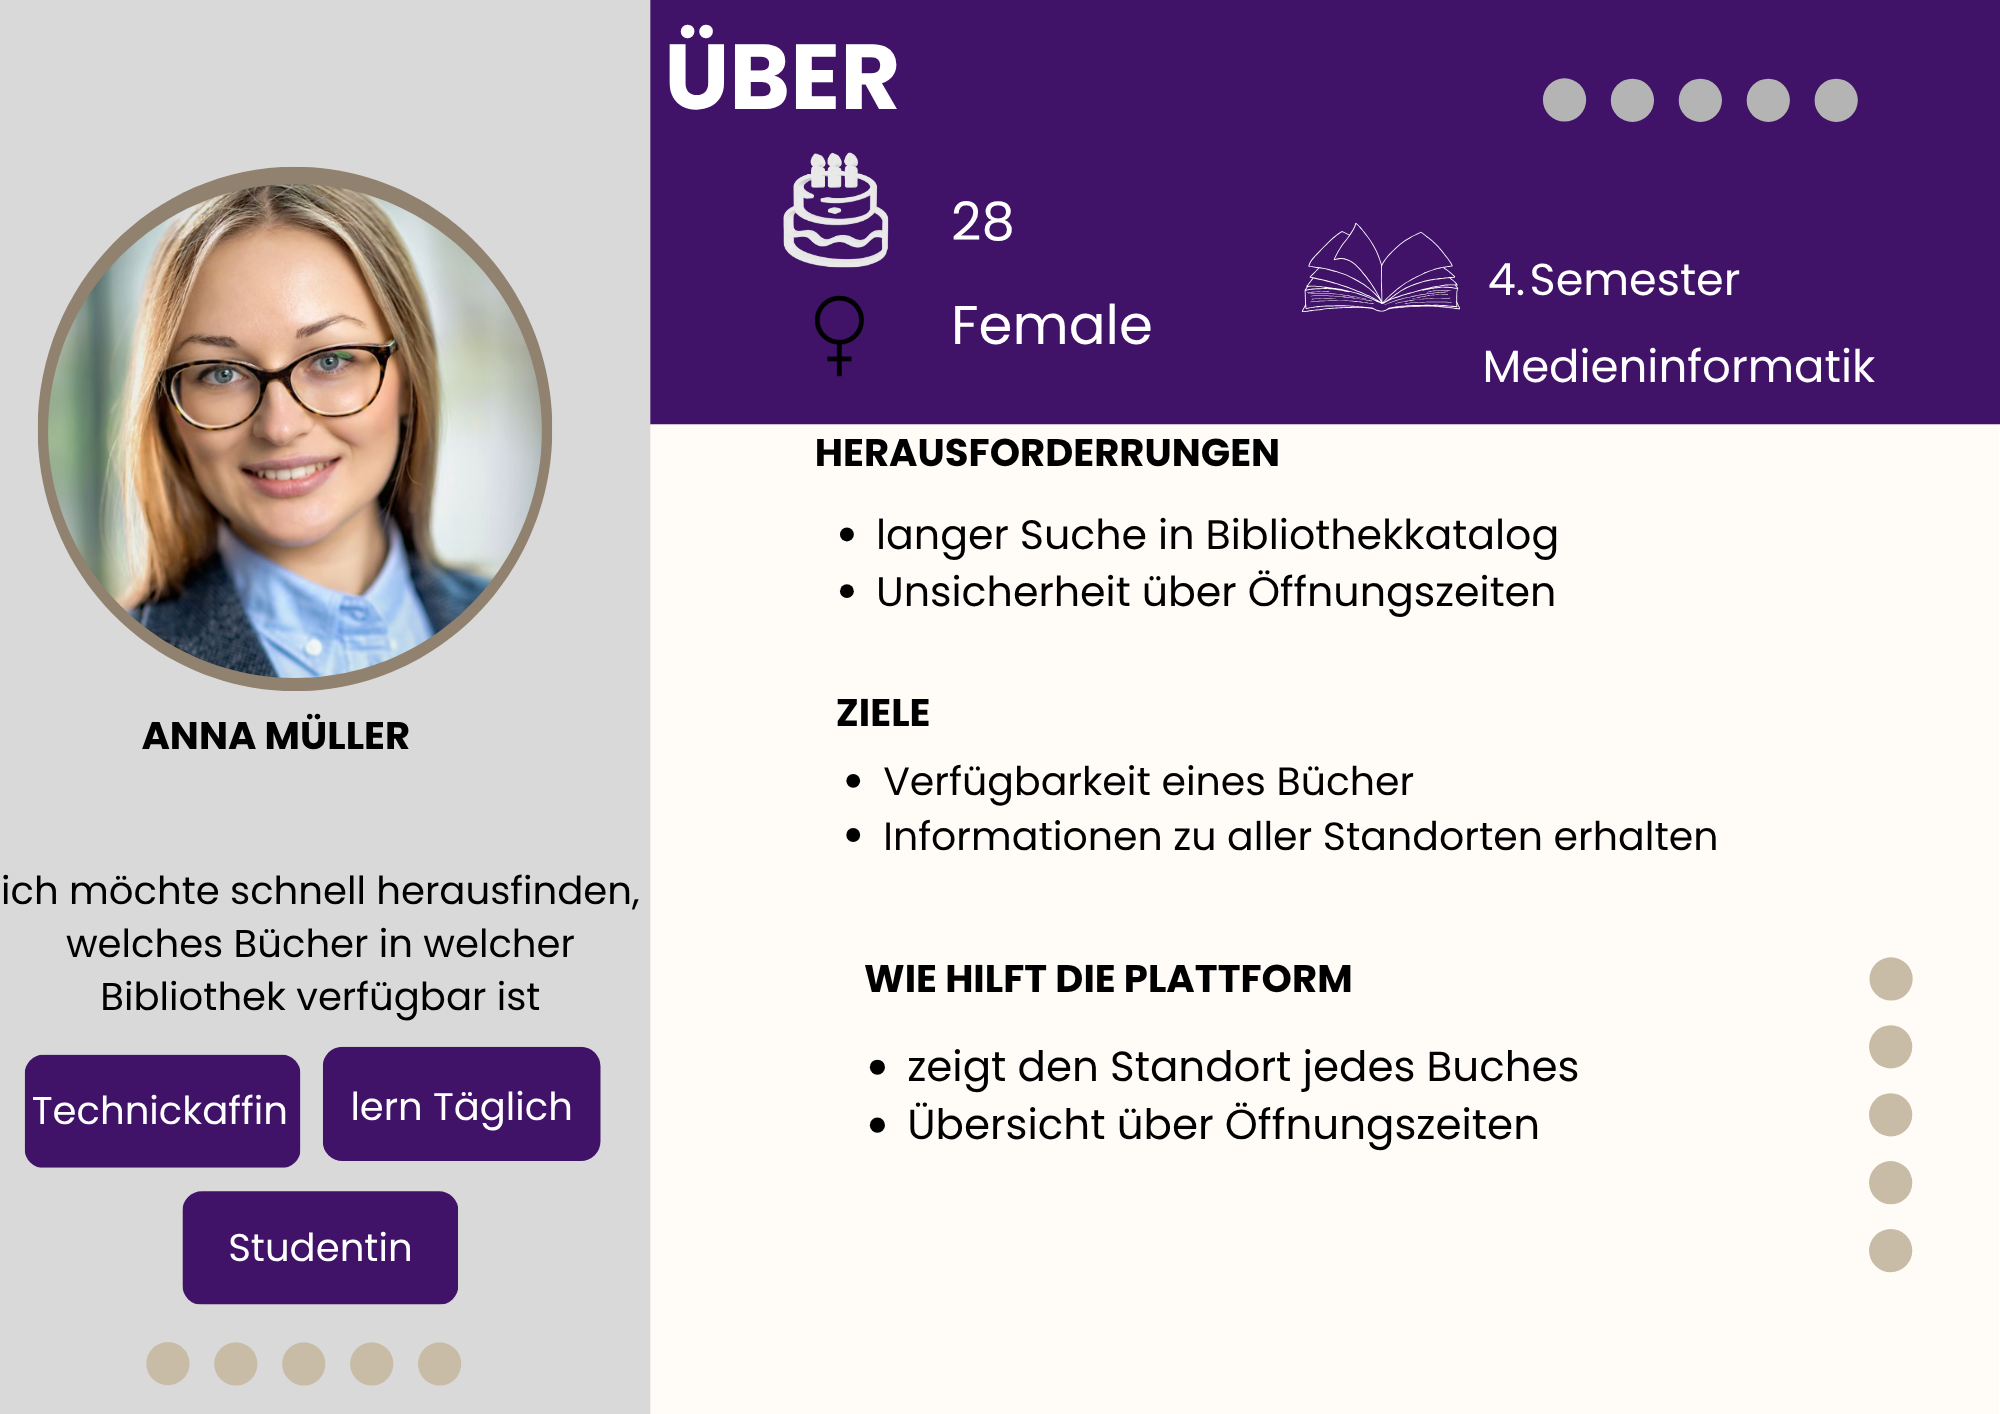
\includegraphics[width=0.9\linewidth]{src/abbildungen/persona1.png}
    \caption{Persona 1}
\vspace{-15pt}
\end{figure}
\begin{figure}[H]
  \centering
   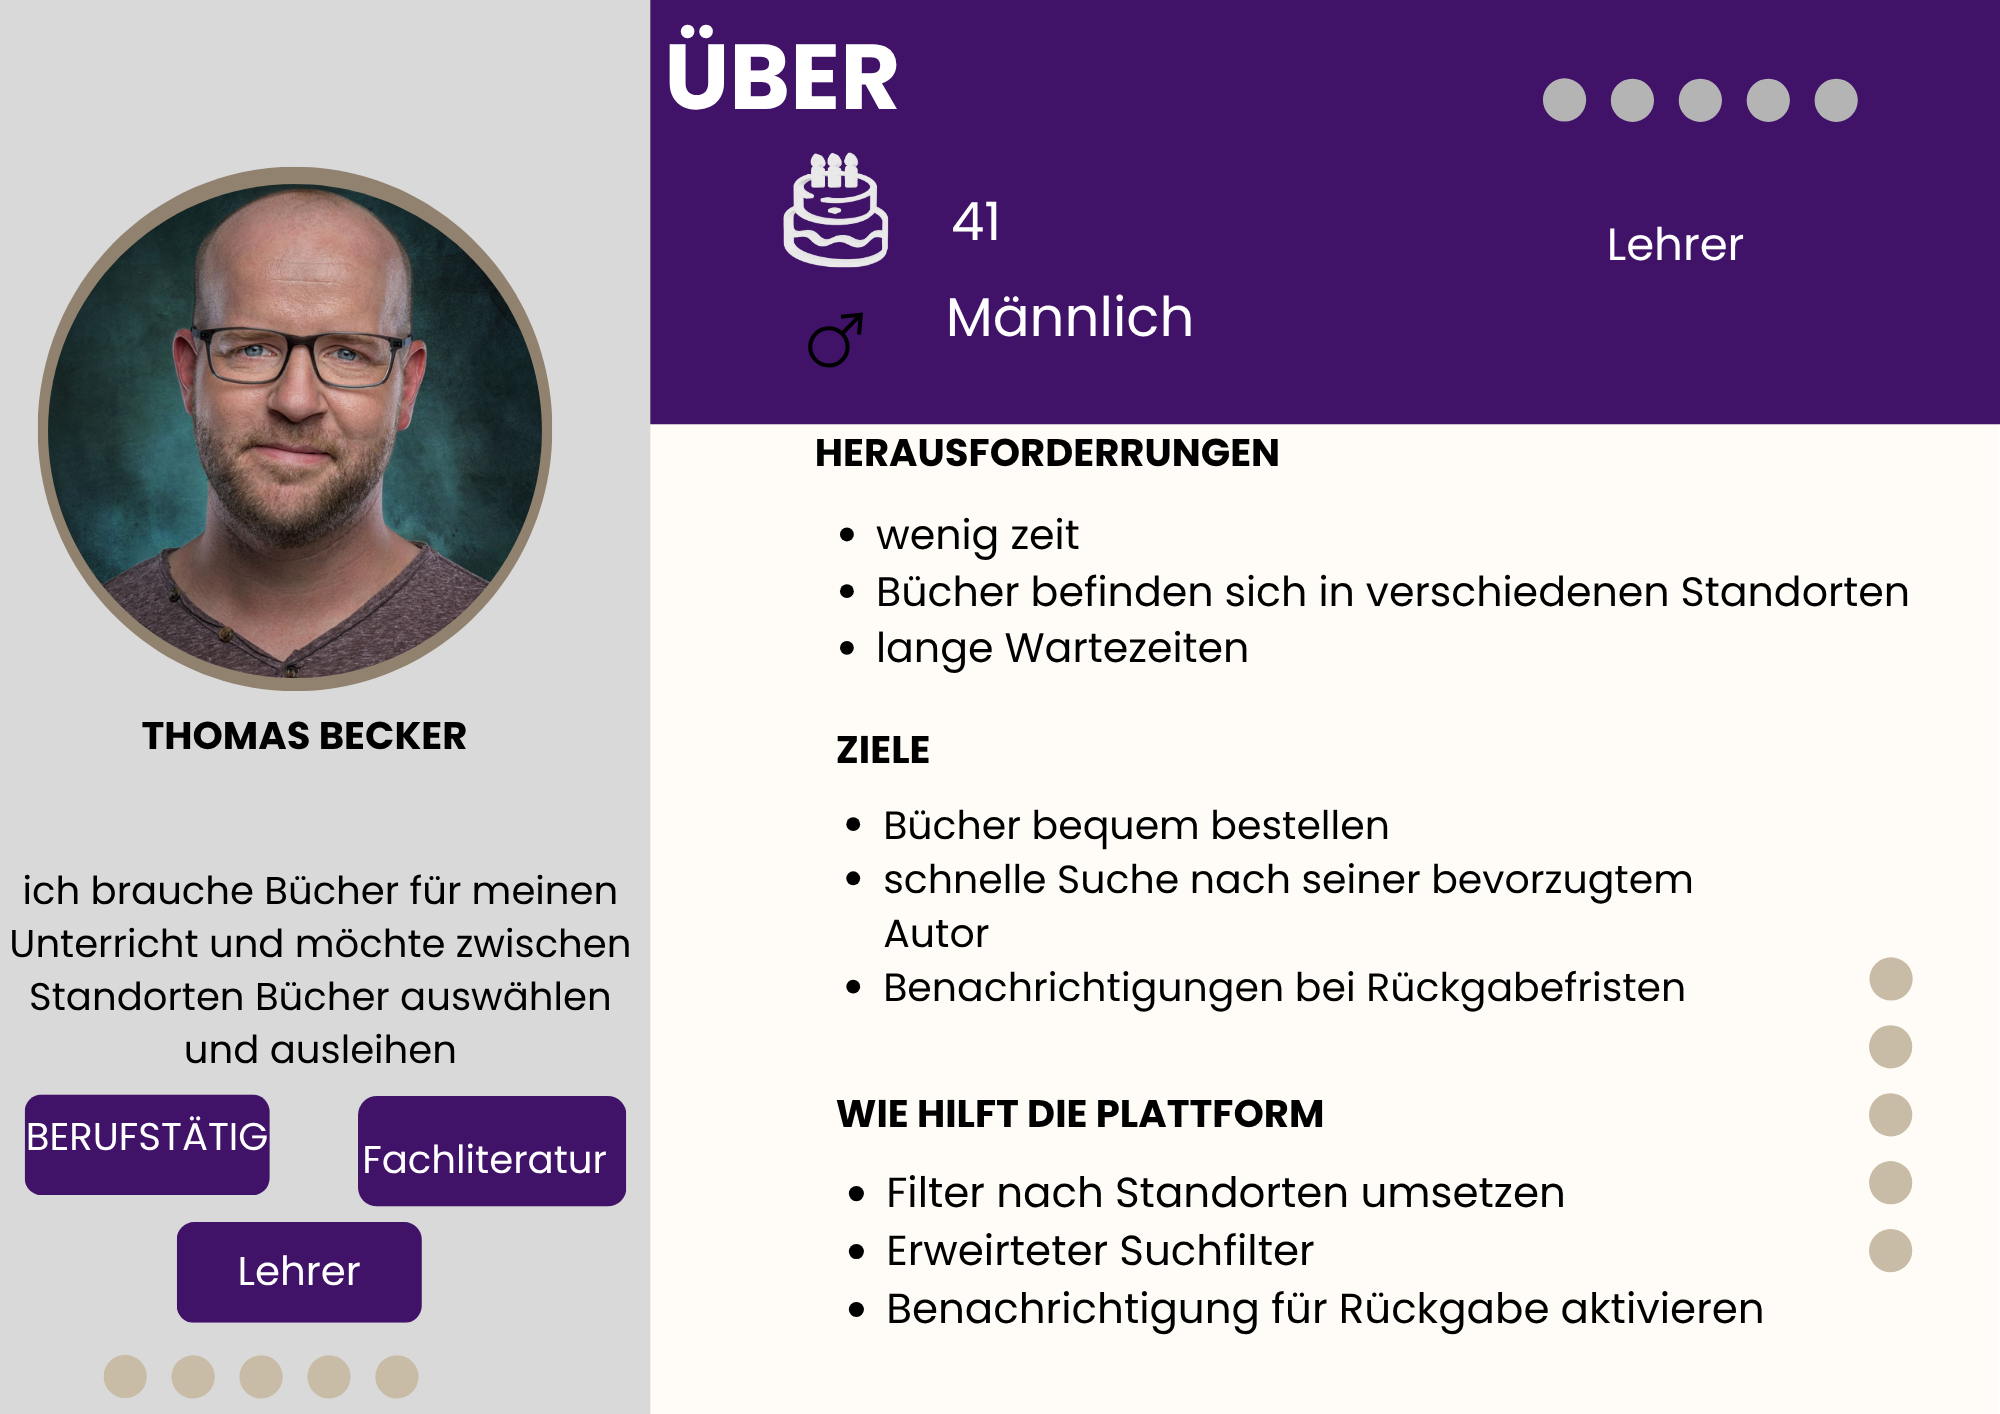
\includegraphics[width=0.9\linewidth]{src/abbildungen/persona2.png}
    \caption{Persona 2}
\vspace{-15pt}
\end{figure}

\subsection{Anforderungsanalyse}
\subsubsection{Funktionale Anforderungen}

\textbf{Mitglieder:}
Mitglieder können sich registrieren und einloggen. Auch ohne Anmeldung ist es möglich,
Bücher zu suchen und deren Verfügbarkeit nach Standort und Regal einzusehen.
Nach dem Login haben Mitglieder Zugriff auf ihre aktiven Ausleihen mit Fälligkeitsdatum
und anfallenden Mahngebühren sowie auf ihre Ausleihhistorie.
Gesperrte Mitglieder erhalten eine Anzeige mit dem jeweiligen Sperrgrund.

\textbf{Mitarbeiterinnen und Mitarbeiter:}
Mitarbeitende authentifizieren sich mit E-Mail, Passwort und Mitarbeiter-ID.
Sie erfassen Ausleihen, indem sie die Ausweisnummer des Mitglieds und mehrere
Barcodes nacheinander einscannen und die Ausleihe anschließend bestätigen.
Bei der Rückgabe können mehrere Bücher gleichzeitig bearbeitet werden,
wobei der Zustand jedes Buches erfasst wird. Mahngebühren werden automatisch
mit 0{,}10~Euro pro Tag nach Ablauf der Leihfrist berechnet.
Darüber hinaus können Mitarbeitende Mitglieder suchen, ihre Ausleihhistorie einsehen
sowie Mitglieder manuell mit Angabe eines Grundes sperren oder freigeben.

\textbf{Administratorinnen und Administratoren:}
Admins haben Zugriff auf eine Übersicht mit Kennzahlen wie Bestand, aktive Ausleihen,
überfällige Ausleihen und gesperrte Mitglieder. Sie können Bücher suchen,
hinzufügen -- mit Angabe von Autor, Standort, Regalnummer und Exemplaranzahl --
sowie aus dem Bestand entfernen. Zusätzlich stehen Autorenstatistiken,
gefilterte Mitgliederübersichten und Auswertungen nach Zeitraum zur Verfügung.

\subsubsection{Nicht-funktionale Anforderungen}

\textbf{Sicherheit:}
Authentifizierung erfolgt sitzungsbasiert; Session Fixation wird verhindert.
Der Zugriff auf geschützte Seiten wird serverseitig durch einen Servlet-Filter (\texttt{MyFilter}) geregelt.
Nicht autorisierte Zugriffsversuche werden auf die Login-Seite umgeleitet.

\begin{figure}[H]
\vspace{-10pt}
  \centering
   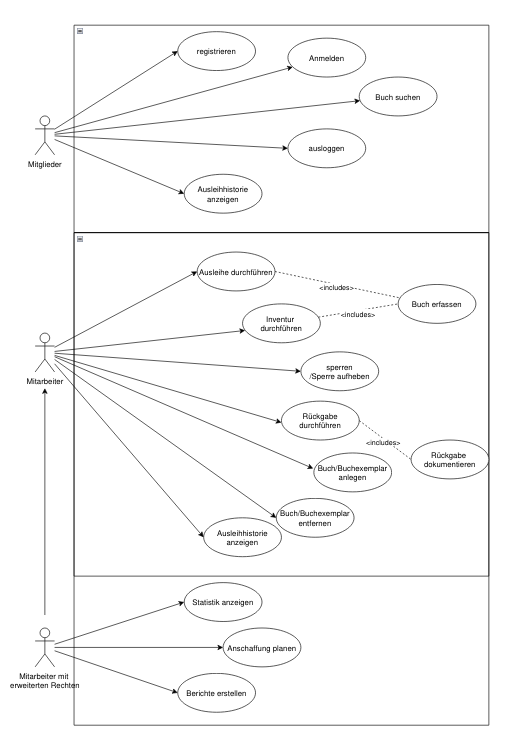
\includegraphics[width=0.9\linewidth]{src/abbildungen/usecase_swe2.png}
    \caption{Use Case}
\vspace{-15pt}
\end{figure}

    \section{Design pattern}
Design Patterns bezeichen Linien von Code, die immer wieder genutzt werden, um gewisse Lösungen für auftretende Probleme oder Herausforderungen in der Softwareentwicklung zu gewährleisten. Durch den Einsatz von Design Patterns wird der Code übersichtlicher, besser wartbar und leichter erweiterbar.
  In unserer Anwendung haben wir das Pattern \textbf{Singelton} umgesetzt, das zur Erzeugungsmuster-Kategorie gehört.\autocite{pattern2026}
  "Das Singleton Pattern stellt sicher, dass von einer Klasse nur eine einzige Instanz existiert und bietet einen globalen Zugriffspunkt auf diese Instanz"\; beschreibt (\citeauthor{pattern2026}, \citeyear{pattern2026}).   
  \begin{minted}{java}
    public class DesignServlet extends HttpServlet{
      private DataSource ds;

      @Override
      public void init() throws ServletException {
        try {
          Context ctx = new InitialContext();
          ds = (DataSource) ctx.lookup("java:/comp/env/jdbc/mariadb");
        } catch (Exception e) {
          throw new ServletException(e);
        }
      }
      @Override
      public void doGet(HttpServletRequest req, Http
      ServletResponse res)
      throws ServletException, IOException {
      connection con = ds.getConnection();
    }
  }
  \end{minted}
Datasource wird in unserer Webanwendung zentral verwendet, auf den alle Servlet zugreifen können. Somit werden Ressourcen gespart, da bei jeder Anfrage nicht mehr direkt neue Datenbankverbindungen aufgemacht werden müssen.


    \section{Analyse Muster von Heide Balzert}
\textbf{Heide Balzert} (* 31 Januar 1955 in Essen) ist eine deutsche Informatikerin und Profesorin im Bereich \textbf{Softwaretechnik und Systemanalyse}. In eines ihrer Bücher \textbf{"Lehrbuch der Objektmodellierung"} untersucht sie verschiedene AnalyseMuster und Beispielanwendungen, uns interessiert prinzipiell der Muster nach dem \textbf{Exemplartyp}. Balzert beschreibt den Exemplartyp als
\begin{itemize}
  \item{Einfache Assoziation}
  \item{erstellte Objektverbindungen nicht verändert werden und werden nur gelöscht, wenn das betrefende Exemplar gelöscht wird}
  \item{Name der neuen Klasse enthält oft Begriffe wie Typ, Gruppe und Beschreibung}
\end{itemize}
Dieses Muster untersucht das Problem, dass mehrere Objekten zum gleichen Typ gehören und gemeinsame Eigenschaften besitzen. Laut der \textit{UML-Diagramm in dem Buch} werden verschiedene Buchexemplare dargestellt, die gleiche Buchbeschreibungen haben. Balzert sprach vom Redundante Speicherung von Attributwerten, da die in der Klasse gespeicherten Informationen immer wieder wiederholt werden. Die Abbildung eine zweite Klasse, die die Eigenschaften \textit{Titel, Autor und Verlag} als Attributen enthält während Buchexemplar \cite{Balzert1955} nur Daten für diese Exemplare besitzt, bildet eine Lösung füür das oben genannte Problem. Durch diese Lösung können Redundanzen vermieden werden und somit ist das Modell übersichtlicher.


    \section{Architekturbild \& Buildprozess}
Die Anfragen werden vom Browser über HTTPS an den \textbf{HAProxy}-Loadbalancer gesendet. Dieser verteilt sie an den Docker-Container, in dem \textbf{Tomcat} als Application-Server läuft. Tomcat verarbeitet die Anfragen und greift dabei auf \textbf{Redis} als Warteschlange für Hintergrundaufgaben sowie über \textbf{JDBC} auf die \textbf{MariaDB} zur persistenten Datenspeicherung zu. Links unten ist die Entwicklungsumgebung mit der Verzeichnisstruktur \textit{(bin/, build/, src/, app/, target/ und local/)} dargestellt. Von dort aus wird die Anwendung erstellt (Build) und über den \textbf{Tomcat Manager} im Docker-Container bereitgestellt (Deploy).
\begin{figure}[H]
  \centering
  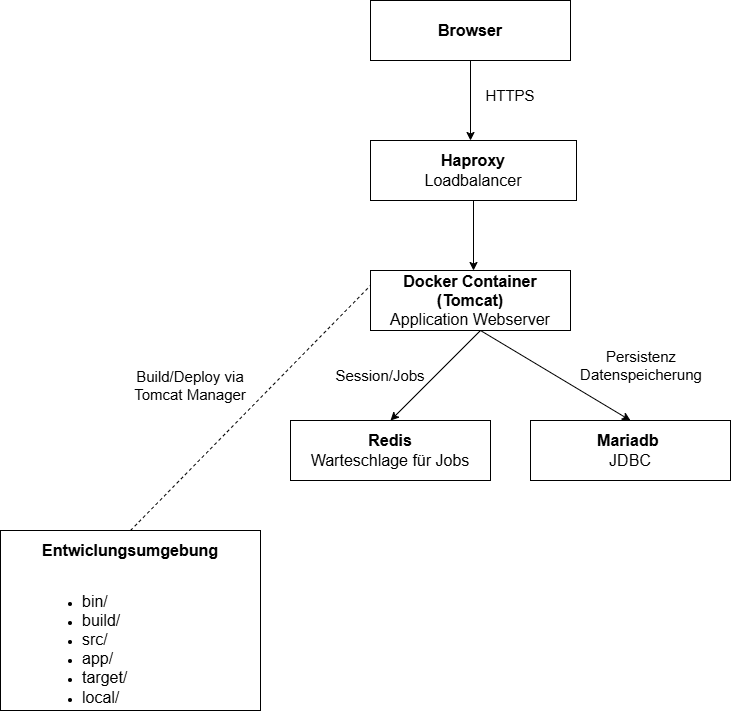
\includegraphics[width=1\linewidth]{src/abbildungen/Architektur.png}
  \caption{Architekturbild}
\end{figure}
    \textbf{Buildprozess:}
   \begin{center}
     \centering
     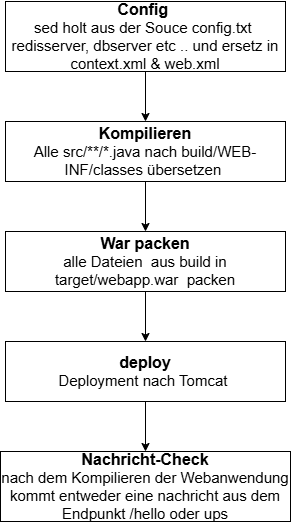
\includegraphics[width=0.9\linewidth]{src/abbildungen/struktur.png}
     \captionof{figure}{build-Prozess}
   \end{center}

    \section{Aktivitätsdiagramm}
Wir haben ein Aktivitätsdiagramm erstellt, dass den kompletten Ablauf vom Login über die Ausleihe eines Mitarbeiters zeigt.
\begin{figure}[H]
    \centering
    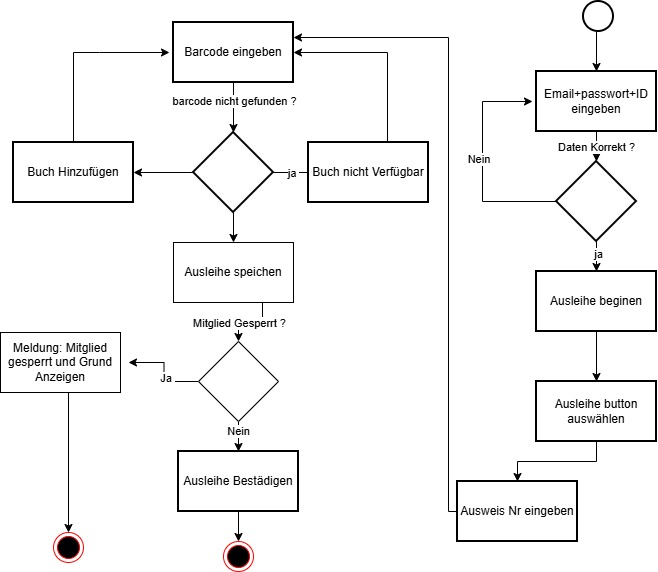
\includegraphics[width=1\linewidth]{src/abbildungen/Swe2_DiagrammD2.jpg}
    \caption{Aktivitätsdiagramm: Login und Ausleihe}
\end{figure}

    \section{Umsetzung \& Kurze Beschreibung}
\subsection{Ausleihe}
Die Ausleihe ist das Herzstück unserer Bibliotheksanwendung. Der Mitarbeiter gibt die Ausweisnummer des Mitglieds ein und scannt anschließend beliebig viele Barcodes der auszuleihenden Bücher. Erst ein Klick auf „Alle ausleihen“ speichert alle Bücher gemeinsam in der Datenbank.
Statt die Bestätigung sofort auszudrucken, wird ein Druckauftrag mit allen Angaben – Mitarbeitername, Ausweisnummer, ausgeliehene Bücher sowie Ausleih- und Rückgabedatum – als eigenständiges Objekt gekapselt und per \texttt{LPUSH} in eine Redis-Warteschlange eingereiht.
\begin{minted}{java}
  while (laeuft) {
    try {
      RedisClient redisClient = JedisAdapter.getClient();
      List<String> antwort = redisClient.brpop(WARTE_SEKUNDEN, QUEUE_KEY);
      if (antwort == null) {
                    continue;
                }
                String auftragAlsText = antwort.get(1);
                schreibeQuittung(auftragAlsText);

            } catch (Exception fehler) {
                System.err.println("Fehler beim Verarbeiten: " + fehler.getMessage());
            }
        }
        System.out.println("DruckWorker beendet.");
\end{minted}
Ein separater \texttt{DruckWorker}-Thread wartet kontinuierlich mit einem blockierenden \texttt{BRPOP} auf neue Aufträge in der Warteschlange, statt die Queue in einer Schleife ständig abzufragen. Sobald ein Auftrag eintrifft, entnimmt der Worker ihn und schreibt die entsprechende Quittung als Textdatei. So bleibt die Ausleihe für den Mitarbeiter sofort abgeschlossen, während das eigentliche „Drucken“ nebenläufig im Hintergrund erfolgt.
\subsection{Rückgabe}
Bei der Rückgabe gibt der Mitarbeiter die Ausweisnummer des Mitglieds sowie beliebig viele Barcodes auf einmal ein, sodass mehrere Bücher in einem Vorgang zurückgenommen werden können. Für jedes Buch prüft die Anwendung automatisch, ob die Rückgabe überfällig ist, und berechnet gegebenenfalls eine Mahngebühr von 10 Cent pro Tag. Wird ein Buch als beschädigt oder verloren gemeldet, sperrt das System das betroffene Mitglied automatisch. Analog zur Ausleihe wird auch hier kein Beleg direkt geschrieben, sondern ein Druckauftrag in dieselbe Redis-Warteschlange eingereiht und vom \texttt{DruckWorker} verarbeitet.
\begin{minted}{java}[h]
long tageUeberfaellig = ChronoUnit.DAYS.between(faellig, heute);
double gebuehr = tageUeberfaellig > 0 ? tageUeberfaellig * 0.10 : 0.0;
if (!zustand.equals("GUT")) {
    PreparedStatement psSperr = con.prepareStatement(
        "UPDATE mitglied SET gesperrt=TRUE, sperr_grund=? WHERE id=?");
    psSperr.setString(1, "Buch " + zustand.toLowerCase() + " zurueckgegeben");
    psSperr.setLong(2, mitglied_id);
    psSperr.executeUpdate();
}
\end{minted}
Beide Prüfungen laufen automatisch im Hintergrund ab: Der Mitarbeiter muss weder die Gebühr selbst berechnen noch manuell entscheiden, ob ein Mitglied gesperrt werden soll. Die Sperrung erfolgt dabei unabhängig von der Gebühr allein aufgrund des gemeldeten Buchzustands.

    \subsection{Registrierung und Login}
Das Klassendiagramm zeigt die drei zentralen Servlets für Registrierung und Anmeldung: \texttt{RegisterServlet}, \texttt{MitgliedLoginServlet} und \texttt{MitarbeiterLoginServlet}. Alle drei erben von \texttt{HttpServlet} und greifen über eine gemeinsame \texttt{DataSource} auf dieselbe MariaDB-Datenbank zu. Das \texttt{RegisterServlet} überschreibt \texttt{doPost()}, da die Registrierungsdaten per POST übertragen werden; die beiden Login-Servlets überschreiben stattdessen \texttt{doGet()}, um die eingegebenen Anmeldedaten zu verarbeiten.
\begin{figure}[H]
    \centering
    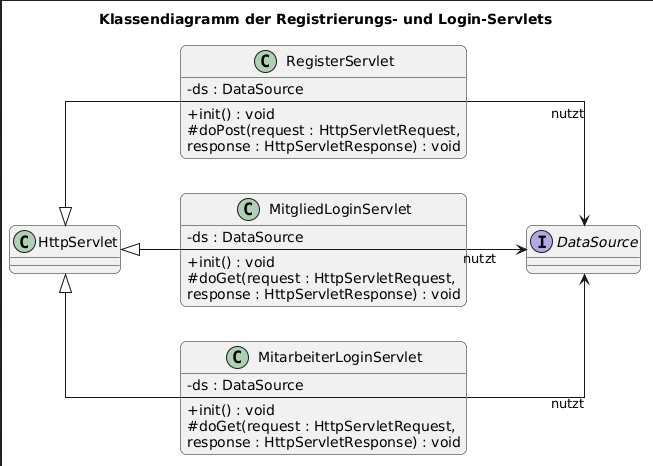
\includegraphics[width=1\linewidth]{src/abbildungen/Poster_Klassendiagramm.png}
    \caption{Klassendiagramm: RegisterServlet, MitgliedLoginServlet und MitarbeiterLoginServlet}
\end{figure}
Das \texttt{RegisterServlet} prüft zunächst, ob alle Eingaben vollständig sind und die beiden E-Mail-Felder übereinstimmen. Da zum Zeitpunkt des Einfügens die künftige Datenbank-ID noch nicht bekannt ist, wird das Mitglied zunächst mit einem Platzhalter für die Ausweisnummer angelegt und diese anschließend anhand der automatisch generierten ID nachgetragen. Die gesamte Operation läuft innerhalb einer Transaktion: Tritt ein Fehler auf, wird sie vollständig zurückgesetzt, sodass kein Mitglied mit unvollständigen Daten in der Datenbank verbleibt.
\begin{minted}{java}[h]
insertStmt.setString(5, "TEMP");
insertStmt.executeUpdate();
long generatedId;
try (ResultSet keys = insertStmt.getGeneratedKeys()) {
    keys.next();
    generatedId = keys.getLong(1);
}
String ausweisnummer = String.format("M-%06d", generatedId);
try (PreparedStatement updateStmt = connection.prepareStatement(
        "UPDATE mitglied SET ausweisnummer = ? WHERE id = ?")) {
    updateStmt.setString(1, ausweisnummer);
    updateStmt.setLong(2, generatedId);
    updateStmt.executeUpdate();
}
connection.commit();
\end{minted}
Das \texttt{MitgliedLoginServlet} vergleicht die eingegebene E-Mail-Adresse und das Passwort mit den gespeicherten Daten. Bei erfolgreicher Anmeldung wird eine Session mit Mitglieds-ID, Ausweisnummer und Rolle angelegt, bevor das Mitglied auf sein Dashboard weitergeleitet wird. Das \texttt{MitarbeiterLoginServlet} funktioniert nach demselben Prinzip, leitet nach erfolgreicher Anmeldung jedoch abhängig von der Rolle entweder auf die Administrator- oder auf die Mitarbeiterseite weiter.

    \section{Lasttest}
Der Lasttest simuliert eine realistische Nutzungslast auf dem System.
Jeder parallele Prozess führt dabei einen vollständigen Ablauf durch:
Login als Mitarbeiter, Rückgabe eines Buches und anschließender Logout.
Jeder Mitarbeiter arbeitet mit einem eigenen Mitglied und Barcode,
um Konflikte zu vermeiden. Die Gesamtdauer wird in Millisekunden gemessen
und zusammen mit der Anzahl erfolgreicher und fehlgeschlagener Anfragen
in einer CSV-Datei gespeichert. 
\begin{figure}[H]
     \centering
     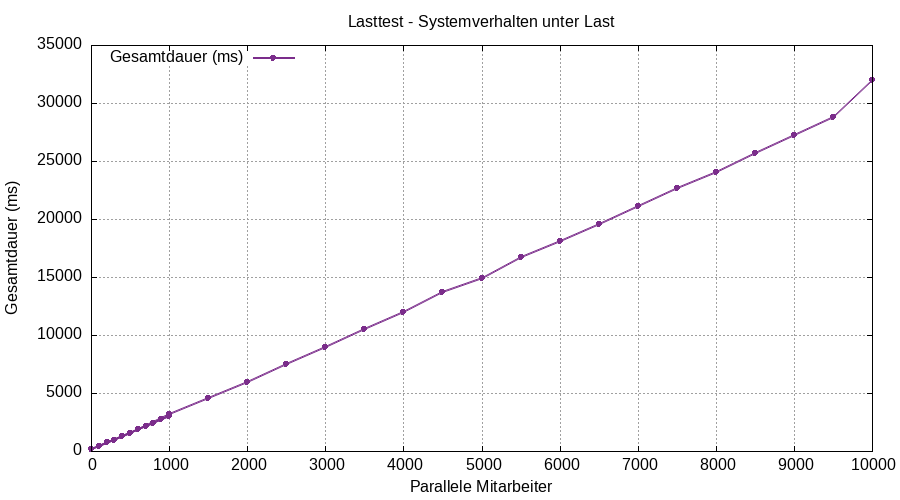
\includegraphics[width=1\linewidth]{src/abbildungen/lasttest.png}
     \caption{Lasttest}
   \end{figure}

   Eine nahezu lineare Kurve zeigt, dass die Infrastruktur (Tomcat, DB-Verbindungspool) auch unter steigender Last stabil und ohne Sättigung skaliert.

    \section{GitHook}

Ein pre-push-Hook prüft vor jedem git push automatisch alle Java-Dateien im Repository mit Checkstyle. Enthält eine Datei Formatierungsfehler, wird der Push abgebrochen.

\begin{minted}{java}[h]
for file in $(find "$ROOT/brotundbutter-sessions-redis-mariadb/src" -name "*.java"); do
  result=$(java -jar "$CHECKSTYLE" -c "$CONFIG" "$file" 2>&1)
  if echo "$result" | grep -q "ERROR"; then
    echo "Formatierungsfehler in: $file"
    FEHLER=1
  fi
done

if [ $FEHLER -eq 1 ]; then
  echo ""
  echo "Push abgebrochen. Bitte Formatierungsfehler beheben."
  exit 1
fi
\end{minted}


    \section{Zusammenfassung}

%Durch dieses Projekt hatten wir die Möglichkeit, unser Wissen und unseren Umgang mit Software Engineering praktisch anzuwenden. Während der Vorlesungszeit haben wir uns mit wesentlichen Themen beschäftigt, die uns dabei geholfen haben, eine strukturierte Webanwendung zu entwickeln und die Anforderungen systematisch zu erfassen. Mithilfe von Personas, Anforderungsanalysen, Use-Cases sowie Aktivitätsdiagrammen konnten wir die wichtigsten Anforderungen der Anwendung darstellen und anschließend in die Implementierung überführen. Durch die Kombination von Servlets, MariaDB und Redis konnten wir die Geschäftslogik umsetzen, Datenbankzugriffe effizient gestalten und eine Warteschlange für die Druckaufträge realisieren. Zusätzlich haben wir ein Design Pattern ausgewählt, analysiert und in unserer Anwendung umgesetzt. Dabei entschieden wir uns für das \textbf{Singleton Pattern}, welches beispielsweise für die zentrale Verwaltung bestimmter Ressourcen eingesetzt werden kann. Durch die Verwendung von vorbereiteten SQL-Anweisungen konnten wir außerdem Sicherheitsrisiken wie \textbf{SQL-Injection} vermeiden. Darüber hinaus beschäftigten wir uns mit den von Balzert beschriebenen Analysemustern und deren UML-Darstellungen. Dabei konnten wir mögliche Probleme innerhalb eines Systems erkennen und passende Lösungsansätze anhand der Muster untersuchen. Um die Qualität unseres Quellcodes sicherzustellen, integrierten wir einen Git-Hook, der vor jedem Push überprüft, ob der Java-Code den festgelegten Formatierungsregeln entspricht. Dadurch konnten Fehler bereits frühzeitig erkannt und verhindert werden, dass fehlerhafter Code in das gemeinsame Repository gelangt. Ein weiterer wichtiger Bestandteil des Projekts war die Durchführung von Lasttests. Hierfür entwickelten wir Testszenarien, welche typische Benutzeraktionen wie Anmeldung, Ausleihe und Abmeldung simulieren. Die daraus gewonnenen Messwerte wurden anschließend visualisiert und analysiert, um das Verhalten der Anwendung unter paralleler Belastung besser beurteilen zu können. Durch die Umsetzung des Projekts konnten wir außerdem wichtige Erfahrungen im Bereich der \textit{Qualitätssicherung} sammeln. Wir haben gelernt, dass Softwarequalität nicht nur durch funktionierende Implementierungen entsteht, sondern durch ein Zusammenspiel verschiedener Maßnahmen wie automatisierten Tests, Code-Qualitätsprüfungen, Versionsverwaltung, Sicherheitsbetrachtungen und Performanceanalysen. Besonders die Integration von Prüfmechanismen in den Entwicklungsprozess hat uns gezeigt, wie Fehler frühzeitig erkannt und die Wartbarkeit einer Anwendung langfristig verbessert werden kann.
%Zusammenfassend konnten wir durch dieses Projekt viele theoretische Inhalte aus dem Bereich Software Engineering praktisch anwenden und ein besseres Verständnis dafür entwickeln, wie komplexe Softwaresysteme geplant, entwickelt, getestet und kontinuierlich verbessert werden.

Durch dieses Projekt konnten wir wesentliche Konzepte des Software Engineerings
praktisch anwenden. Mithilfe von Personas, Anforderungsanalysen, dem Use-Case und dem
Aktivitätsdiagram wurden die Anforderungen systematisch erfasst und in eine
strukturierte Webanwendung überführt. Die Kombination aus Servlets, MariaDB und
Redis ermöglichte eine effiziente Umsetzung der Geschäftslogik sowie eine
Druckwarteschlange nach dem Producer-Consumer-Muster. Zur Qualitätssicherung
integrierten wir einen Git-Hook, der vor jedem Push die Java-Formatierung prüft,
sowie Lasttests, die das Systemverhalten unter paralleler Belastung analysieren.
Das Projekt hat gezeigt, dass Softwarequalität durch das Zusammenspiel von
Implementierung, Sicherheit, Versionsverwaltung und Performanceanalyse entsteht.

    
    % Literaturverzeichnis anzeigen
    \section*{Referenzen}
    \vspace*{0.3cm}
    \printbibliography[heading=none]

  \end{multicols*}
\end{document}

